\section{РЕАЛИЗАЦИЯ}

Проанализировав все вышеперечисленные программы 

Таким образов в программу вошли классические алгоритмы численных методов, такие как методы матричной алгебры, методы
Ньютона и так далее. Для её написания были использованы \textit{язык программирования C++}, \textit{фреймворк QT} и система сборки
проектов \textit{CMake} \ref{fig:stack}.
Для поиска ошибок и утечек памяти применилась связка из отладчика \textit{GDB} и профилировщика \textit{Valgrind}. 

\begin{figure}
    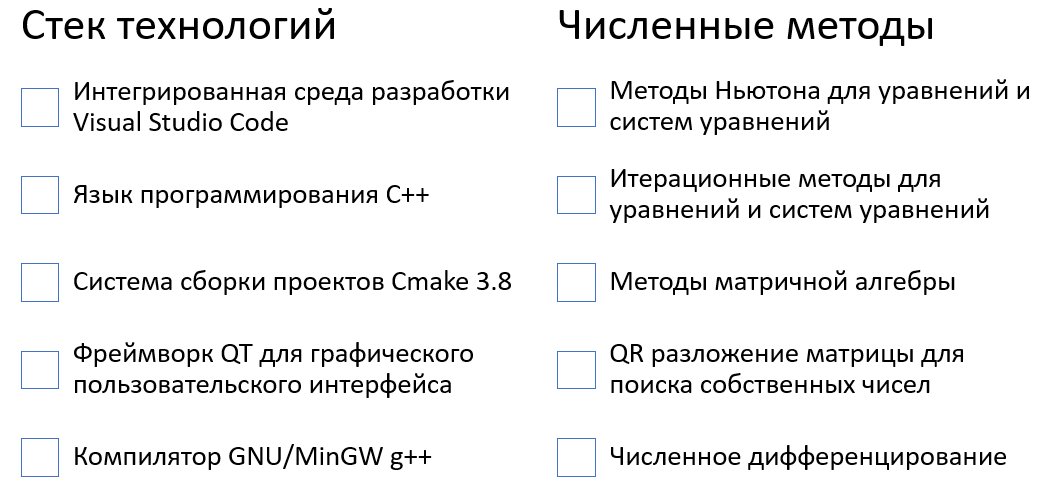
\includegraphics[width=15cm]{2-04-realisation}
    \caption{Технологии и алгоритмы}
    \label{fig:stack}
\end{figure}

В данной программе реализован большой перечень как явных так и неявных методов с различным порядком точности.

%Для повышения порядка точности явных методов используется процедура Рунге-Ромберга, заключающаяся в повторном решении в точке с вдвое меньшим шагом и сравнении с предыдущим.

%Если погрешность сильно меньше заданной точности, что шаг интегрирования стоит уменьшить, если же больше, что увеличить.

%и вложенные методы. Неявные и их виды ()нулевая строка, нулевой столбец, диагональные, полные) параллельные

\textbf{Вычисление жёсткости}

Коэффициентом жёсткости задачи называется отношение максимального модуля действительной части собственных чисел матрицы системы к
минимальной при условии, что все действительные части собственных чисел меньше нуля.

Для вычисления коэффициента жёсткости сначала по данной задаче строится матрица-система. Собственные числа данной матрицы находятся
при помощи алгоритма QR-разложения.

дополнительные методы ()кью-ар
методы решения слау

%методы решения

Для неявных методов используются алгоритмы итераций Ньютона, Зейделя и простой итерации.

%алгоритмы работы с матрицами

Кью-Ар разложение 

хоть метод ньютона и второго порядка но применим и для методов

\textbf{Описание работы программы}

%картинка стека технологий

\textbf{Парсер математических выражений}

При режиме работы с задачей Коши от пользователя требуется ввести задачу и аналитическое решение (при наличии). 

Для обработки строки с задачей используется парсер математических выражений. Проводится лексический анализ строки и строится дерево
математических выражений, содержащее функции в качестве узлов и числовые константы с переменными в качестве листьев. Интерфейс парсера
позволяет использовать его как функтор, принимающий либо одну переменную, либо массив переменных. 

%Далее последует выбор метода решения и точности. В результате работы генерируется pdf-отчёт с краткой постановкой задачи, подробным
%описанием метода решения и таблицы Бутчера, используемой методом, В конце отчёта представлен график с сравнением точного и численного
%решения.

%лексический анализ, жёсткость, выбор метода, построение методов.
%сравнение по времени лексического анализа и встроенных функций
%скрины интерфейса

%==================================

%Программа представляет из себя набор модулей

%форма для вывода/ввода
